\documentclass[11pt]{report}
\usepackage[french]{babel}
\usepackage{graphicx}
\usepackage[utf8]{inputenc}
\usepackage{float}
\usepackage{array}
\usepackage{tabularx}
\usepackage[T1]{fontenc}
\usepackage{xcolor}
\usepackage{multirow}
\usepackage{titlesec}
\usepackage{titletoc}
\usepackage{setspace}

\def\code#1{\texttt{#1}} % pour écrire du code (police monospace)
\def\comment#1{\color{gray} #1 \color{black}}

\begin{document}
\renewcommand{\labelitemi}{$\bullet$}
\renewcommand{\labelitemii}{$\circ$}
\thispagestyle{empty}

\titleformat{\chapter}[display]
	{\normalfont\bfseries}
	{}
	{-3.5ex}
	{
	\Huge}
	[]

\titlecontents{chapter}[0em]
	{\vskip 1ex}%
	{\bfseries\large}% numbered sections formattin
	{\itshape}% unnumbered sections formatting
	{\bfseries \titlerule*[4pt]{.}\contentspage}%
	[{\vskip 1ex}]
	
\titlecontents{section}[4em]
	{\vskip 0.5ex}%
	{\contentslabel{2.3em}}% numbered sections formattin
	{}% unnumbered sections formatting
	{\titlerule*[4pt]{.}\contentspage}%
	[{\vskip 0.5ex}]
	
\titlecontents{subsection}[8em]
	{\vskip 0.25ex}%
	{\contentslabel{2.3em}}% numbered sections formattin
	{}% unnumbered sections formatting
	{\titlerule*[4pt]{.}\contentspage}%
	[{\vskip 0.25ex}]

\begin{center}
	\huge  \bf Rapport du TP4: Paralèlliser un algorithme de filtrage numérique basé
	sur des opérations de convolution avec OpenCL et OpenACC\\
	\vfill

	\Large Equipe numéro 2\\
	\vspace*{3ex}

	\medskip
	\normalsize
	\textit{Houssem Sebouai}\\
	111 134 915\\
	houssem.sebouai.1@ulaval.ca\\
	
	\medskip
	\normalsize
	\textit{Thierry St-Gelais}\\
	111 169 338\\
thierry.st-gelais.1@ulaval.ca\\

	\vfill
	Dans le cadre des travaux pratiques du cours\\
	\LARGE GLO-7014\\
	\large Programmation parallèle et distribuée\\
	Professeur: Marc Parizeau

	\vfill
	
\includegraphics[width=5cm]{Images/logo.jpg}
	\\
	Hiver 2017
\end{center}

\newpage

\onehalfspace
\tableofcontents
\listoffigures
\newpage
\chapter{Introduction}

	Pour ce quatrième TP, il nous était demandé de paralléliser le code donné lors du TP2 en utilisant non pas le processeur de notre ordinateur, mais bien son GPGPU. Pour la première implémentation nous avions le choix entre CUDA ou bien OpenCL et nous devions utiliser OpenACC pour la seconde implémentation du code parallèle.
	
	\bigskip
	Pour la première implémentation nous avons choisi d'utiliser OpenCL par simplicité, mais aussi par souci de portabilité, CUDA n'étant supporté que par les GPUs de Nvidia.
	
\clearpage
\setcounter{chapter}{0}
\chapter{Implémentation d'OpenCL}

	\section{Description générale de l'algorithme}
		Le fonctionnement de l'algorithme OpenCL est assez complexe. Il y a d'abord la phase d'initialisation des éléments d'OpenCL, soit (dans l'ordre) la platforme, le device, le contexte, la \textit{commandQueue}, les buffers, le programme et finalement le kernel. Entre ces deux initialisation il y a une opération de construction du programme à partir d'un fichier kernel d'OpenCL, qui comprends les instructions qui seront envoyées au GPU.
	
	\section{Approche adoptée pour la parallélisation}
		La méthode utilisée pour paralléliser ce code fut de retirer les deux boucles externes du code séquentiel, puis de faire rouler ce code pour chaque pixel de l'image, c'est-à-dire que les coeurs du GPU lisent qu'un pixel à la fois, le traitent, puis l'inscrivent dans l'image de sortie. Ceci nous permet donc de paralléliser au possible le code.
	
	\section{Expérimentations et résultats}
	
	
		\subsection{Protocole d'expérimentation}
				Malheureusement, la plateforme de test que nous souhaitions utiliser ne supporte pas OpenCL 1.2, qui est nécessaire au traitement des données de type \texttt{double}, telles que celles utilisées. Nous n'avons donc, pour le moment, aucun résultats à présenter.
				
		\subsection{Résultats}
			\textit{voir Protocole d'expérimentation.}
		\subsection{Interprétation}
			\textit{voir Protocole d'expérimentation.}
	
\clearpage
\chapter{Implémentation d'OpenACC}
	
	\section{Description générale de l'algorithme}
		Le fonctionnement général de l'algorithme OpenACC est similaire au code séquentiel, donc quatres boucles imbriquées. Les deux première assurent le parcours de l'image dans les deux dimensions, alors que les deux boucles les plus profondes assurent le parcours du noyau dans les deux dimensions. 
		
		\bigskip
		Au plus profond de ces quatre boucles on retrouve trois opérations, qui nous permettent de déterminer la nouvelle couleur du pixel en cours en y accumulant les valeurs de couleurs des pixels voisins selon un noyau de flou gaussien préalablement défini.
		
		\bigskip
		Plusieurs personnes ont mentionné des problèmes avec OpenACC, notamment le fait que g++ ne le supporte pas. De notre côté, nous avons en effet remarqué quelques soucis avec cette méthode. En activant les optimisations de niveau 3 du processeur, nous avons réussi à obtenir un speedup considérable, de beaucoup supérieur à celui obtenu avec nos résultats du TP2, soit avec OpenMP, ce qui nous pousse à croire que la carte graphique contribuait bel et bien aux calculs, bien qu'elle ne soit pas détectée par la fonction \texttt{acc\_get\_device\_type()}.
		
	\section{Approche adoptée pour la parallélisation }
		Pour paralléliser ces boucles, nous avons décider d'y aller avec l'approche \texttt{parallel} plutôt que \texttt{kernels}, puisque cela nous a permis de nous familiariser un peu plus avec le fonctionnement d'OpenACC.
		
		\bigskip
		Nous avons, à force d'essais et d'erreurs choisi de paralléliser les boucles \og paires \fg{}, c'est-à-dire la 2\textsuperscript{e} et la 4\textsuperscript{e} boucle. Nous avons déterminé après plusieurs tests que c'est ce que nos GPUs supportait le mieux sans subir de ralentissement dû à la compétition des fils d'exécution pour obtenir les ressources (coeurs du GPU).

		\bigskip
		\begin{figure}[H]
			\noindent\texttt{
				\#pragma acc data\\
		        \{\\
		        \hspace*{1em}\#pragma acc parallel\\
		        \hspace*{1em}\{\\
		        \hspace*{1em}\hspace*{1em}for (Largeur de l'image) \{\\
		        \hspace*{1em}\hspace*{1em}\hspace*{1em}\#pragma acc loop private(lRGB)\\
		        \hspace*{1em}\hspace*{1em}\hspace*{1em}for (Hauteur de l'image) \{\\
				\hspace*{1em}\hspace*{1em}\hspace*{1em}\hspace*{1em}//Initialiser le vecteur de couleurs (lRGB) ici.\\       
		        \hspace*{1em}\hspace*{1em}\hspace*{1em}\hspace*{1em}for (Largeur du noyau) \{\\	
		        \hspace*{1em}\hspace*{1em}\hspace*{1em}\hspace*{1em}\hspace*{1em}\#pragma acc loop private(lRGB)\\
		        \hspace*{1em}\hspace*{1em}\hspace*{1em}\hspace*{1em}\hspace*{1em}for (Hauteur du noyau) \{\\
	            \hspace*{1em}\hspace*{1em}\hspace*{1em}\hspace*{1em}\hspace*{1em}\hspace*{1em}//Calculer le niveau de rouge des pixels ici.\\
	            \hspace*{1em}\hspace*{1em}\hspace*{1em}\hspace*{1em}\hspace*{1em}\hspace*{1em}//Calculer le niveau de vert des pixels ici.\\
	            \hspace*{1em}\hspace*{1em}\hspace*{1em}\hspace*{1em}\hspace*{1em}\hspace*{1em}//Calculer le niveau de bleu des pixels ici.\\
		        \hspace*{1em}\hspace*{1em}\hspace*{1em}\hspace*{1em}\hspace*{1em}\}\\
		        \hspace*{1em}\hspace*{1em}\hspace*{1em}\hspace*{1em}\}\\
		        \hspace*{1em}\hspace*{1em}\hspace*{1em}\hspace*{1em}//Placer le résultat dans l'image ici.\\
		        \hspace*{1em}\hspace*{1em}\hspace*{1em}\}\\
		        \hspace*{1em}\hspace*{1em}\}\\
		        \hspace*{1em}\}\\
		        \}\\
	        }
	        \caption{Structure du code OpenACC}
        \end{figure}
        
        \bigskip
        Comme il est possible de voir dans le code précédent, nous avons imbriqué la totalité des boucles dans une région \texttt{data}, afin d'éviter le transfert inutile de données. Nous transférons les dimensions de l'images, ainsi que celle du noyau avec la directive \texttt{copyin}, de façon à ce que celles-ci ne soit disponibles qu'en lecture seul, nous créons de l'espace en mémoire pour le vecteur de couleur avec \texttt{create} et envoyons l'image en lecture/écriture avec \texttt{copy}. À noter que les dimentions ont été regroupées dans un tableau, de façon à ce que leur emplacement en mémoire soit contigu, afin d'optimiser le transfert des données. Le même traitement a été réservé aux valeurs de rouge, vert et bleu.
	
	\section{Expérimentations et résultats}

		\subsection{Protocole d'expérimentation}
				Pour tester les performances du code parallelisé avec OpenACC, nous avons créé un noyau de $19 \times 19$ afin d'augmenter le temps de calcul et avons utilisé une image de dimensions $5444 \times 4083$ pixels.
		
		\bigskip
		Les tests ont été effectués sur un ordinateur portable avec un processeur Intel\textsuperscript{(R)} Core\textsuperscript{TM} i7 Q 720 \@ 1.6 GHz, avec comme GPU une GeForce GT230M.
		
		À chaque itération du test, le programme devait appliquer le flou gaussien 4 fois. Vous verrez sur les graphiques suivants deux comparaisons pour le GPU, une avec la directive \texttt{present\_or\_*} et une sans. On souhaite ainsi voir une (légère) différence de vitesse lorsque le processeur doit transférer les données à chaque fois et lorsque le GPU les garde en mémoire.
		
		\subsection{Résultats}
		
		\begin{figure}[H]
			\centering
			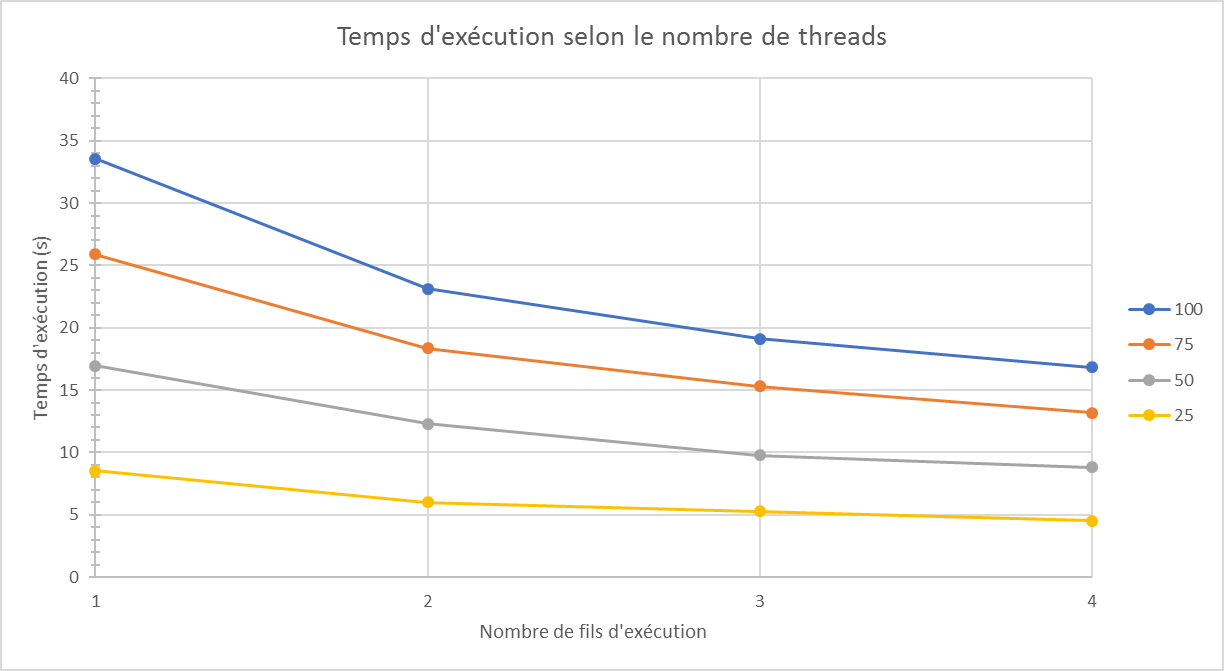
\includegraphics[scale=0.8]{images/graph_temps}
			\caption{Temps d'exécution, flou gaussien}
		\end{figure}
		
		\begin{figure}[H]
			\centering
			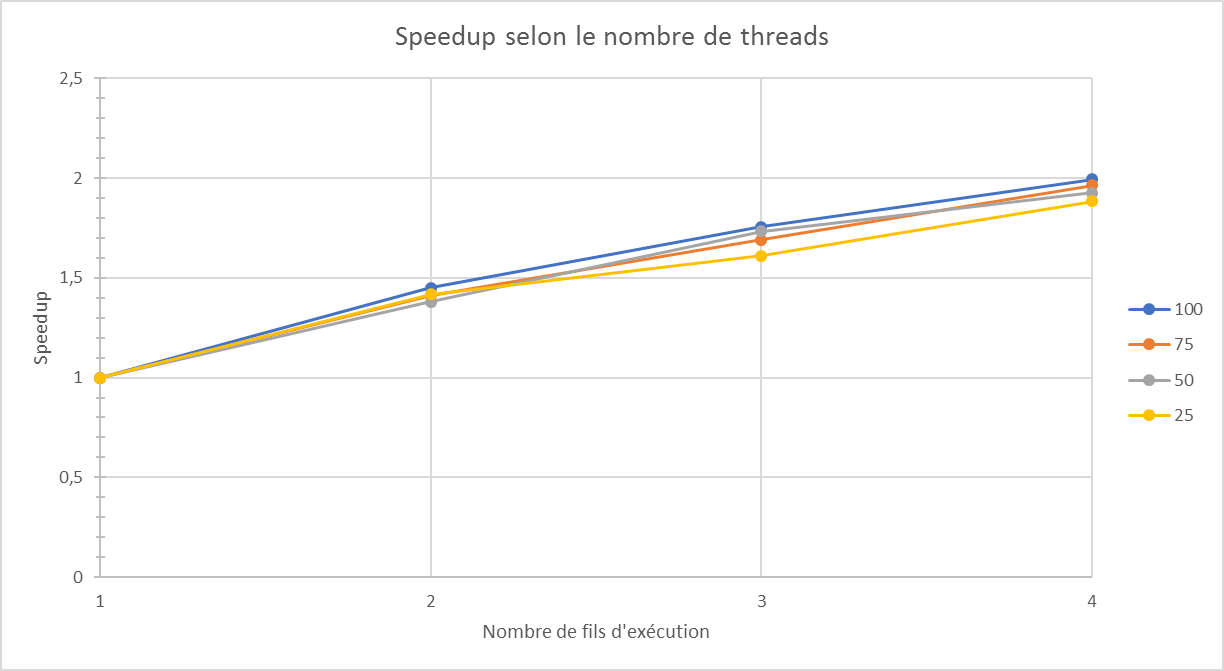
\includegraphics[scale=0.8]{images/graph_speedup}
			\caption{Speedup par rapport au code séquentiel}
		\end{figure}
		
		\subsection{Interprétation}
			Les résultats présentés ci-haut représentent une moyenne de 10 instances de tests réalisés sur la plateforme de test mentionnée plus haut. On peut voir une très légère différence entre les instances où le GPU gradait les éléments en mémoire et où il les transférait à chaque fois, mais cette différence est tellement faible (~10\%) qu'elle peut être attribuée à la marge d'erreur des tests.

			On peut par contre voir un speedup assez monumental d'OpenACC vis à vis l'approche séquentielle, soit un ratio d'environ 74.9. Côte à côte avec OpenMP, OpenACC s'en tire encore une fois très bien, avec un speedup d'environ 30.69.

			Ces résultats nous font penser que malgré les incongruences avec OpenACC, le GPU a joué un rôle certain dans le calcul du flou gaussien, puisqu'un tel speedup aurait été impossible à atteindre avec seulement le CPU, tel que le démontre la différence marquée entre le temps d'exécution avec OpenMP et celui avec OpenACC. De plus, nous nous sommes aperçu qu'en activant les optimisations de processeur de niveau 3(-O3), nous étions en mesure d'obtenir ces résultats, alors qu'en ne les utilisant pas, le code parallélisé avec OpenACC était environ aussi lent, sinon plus que le code séquentiel.
			

\chapter{Conclusion}

	Pour ce travail, il nous était demandé de paralléliser un algorithme de filtrage d'image numérique en utilisant les technologies OpenCL (ou CUDA) et OpenACC.

	\bigskip
	Malheureusement pour nous, notre plateforme de test n'offrait pas le support pour OpenCL 1.2, nécéssaire à l'utilisation des \texttt{double}, ce qui nous a empêché d'obtenir des résultats ou même de tester notre code.

	\bigskip
	Pour ce qui est d'OpenACC, nous avons été en mesure de comprendre comment fonctionnait les directives \texttt{parallel} et \texttt{kernels}, bien que nous n'ayons pas utilisé \texttt{kernels}. Nous avons été en mesure de découvrir que (dans notre cas), les optimisations -O3 du compilateur g++ nous permettaient d'utiliser OpenACC même si, selon la documentation présente en ligne, OpenACC n'était pas supporté par g++, ni même par gcc depuis gcc 5.1.
	
	\bigskip
	Au final, ce projet nous a permis de voir deux facettes de la même médaille, soit la programmation directe des instructions à faire suivre au GPU, avec OpenCL, et l'utilisation de directives de haut niveau cérant ces instructions pour nous, avec OpenACC.

	\bigskip
	Si ce projet était à refaire, nous nous assurerions que nos plateformes soient compatibles avec les technologies à utiliser avant de commencer le projet, nous donnant ainsi une plus grande marge de manoeuvre dans le temps pour corriger le tir.
	
\end{document}
